\chapter{Toolfindung}
\label{ch:toolfindung}

In diesem Kapitel werden vier Tools untersucht, welche \gls{ub} auffinden sollen:
\begin{itemize}
    \item PC-lint Plus \cite{misc:pclintplus}
    \item Cppcheck \cite{misc:cppcheck}
    \item \gls{ubsan} (wird von GCC und Clang++ verwendet) \cite{misc:ubsan}
    \item PVS-Studio \cite{misc:pvsstudio}
\end{itemize}
Die Tools werden dabei anhand einer Bewertungsmatrix mit den Anforderungen F-1 bis F-6, NF-2 und NF-3 bewertet. Die Anforderungen sind mit Zahlen von eins bis fünf gewichtet, wobei 
eine höhere Zahl für eine höhere Relevanz steht. Bei F-1 und F-2 wird das Erfüllen der Anforderung in Form einer Warnung mit 70\% gewertet. 100\% werden vergeben, wenn das Tool einen 
Error ausgibt.
\begin{figure}[htpb]
    \centering
    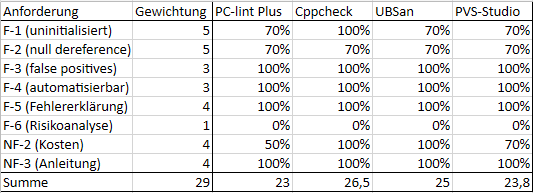
\includegraphics[width=0.8\textwidth]{toolfindung}
    \caption{Bewertungsmatrix}
    \label{img:toolfindung}
\end{figure}

Alle untersuchten Tools geben für F-1 und F-2 eine Warnung aus. Eine Ausnahme bildet dabei Cppcheck, welches für F-1 einen Error ausgibt. \newline
False positives wurden bei durchgeführten Tests von keinem Tool erkannt.
Da jedes Tool von der Kommandozeile aus bedienbar ist, sind alle Tools automatisierbar. Dies ermöglicht auch eine Integration in Projekte jeder Art. Für PVS-Studio existiert jedoch 
zusätzlich eine Extension für Visual Studio \cite{misc:pvsplugin}. \newline
Eine Risikoanalyse wird von keinem Tool zur Verfügung gestellt. \newline
Im Gegensatz dazu verfügt jedes Tool über eine Dokumentation. Beim Aufruf am 02.02.2021 referenzierte die Dokumentation von PVS-Studio (\cite{misc:pvsdoku}) nicht mehr vorhandene Seiten. Zusätzlich 
funktionierte die integrierte Suchfunktion nicht mit einzelnen Wörtern. Dies ist aktuell (letzter Aufruf 16.06.2021) nicht mehr der Fall.\newline
Sowohl Cppcheck als auch \gls{ubsan} sind kostenfrei verfügbar. \newline 
PVS-Studio kostet im ersten Jahr, für ein Entwicklerteam mit 10-30 Entwicklern, 21.000€. Für jedes folgende Jahr belaufen sich die Kosten auf 80\% des Preises (16.800€).\newline 
Die zuständigen Stelle von PC-Lint Plus hat bezüglich auf eine Preisanfrage, zum aktuellen Zeitpunkt, noch keine Rückmeldung gegeben. Aus diesem Grund wird NF-2 bei diesem Tool 
vorläufig mit 50\% bewertet.

\section{Auswahl}
\label{sec:auswahl}

Cppcheck erreicht in der Bewertungsmatrix (Abbildung: \ref{img:toolfindung}) die höchste Punktzahl und ist somit Sieger der Bewertung und daraus resultierend die Toolempfehlung. 
Jedoch zeigen die anderen Tools keine übermäßigen Abweichungen auf und können auch in Betracht gezogen werden, falls beispielsweise eine Integration in Visual Studio gewünscht ist 
(PVS-Studio). \newline
Zur optimalen Toolfindung empfiehlt sich somit das Testen der einzelnen Tools in einem größeren Projektumfeld. Die kostenpflichtigen Tools bieten für diesen Zweck kostenlose 
Testlizenzen an. Attraktiv ist hierbei PVS-Studio, da dieses mit einer Extension in Visual Studio integriert werden kann. Das Tool fällt allerdings durch die vergleichsweise 
schlechte Dokumentation auf. Zusätzlich ist PVS-Studio allgemein weniger bekannt und die Suche nach Online-Hilfe ist somit schwieriger. \newline
Zusätzlich können die kostenfreien Tools zusätzlich zu dem schlussendlich ausgewählten Tool eingesetzt werden. Dies ermöglicht eine höhere Fehlerabdeckung, garantiert allerdings nicht, 
dass neue/mehr Fehler erkannt werden. Da das Einsetzen der kostenlosen Tools nur Zeit kostet, ist der Einsatz dieser immer eine Überlegung wert.